%%%%%%%%%%%%%%%%%%%%%%%%%%%%%%%%%%%%%%%%%%%%%%%%%%%%%%
% A Beamer template for University of Wollongong     %
% Based on THU beamer theme                          %
% Author: Qiuyu Lu                                   %
% Date: July 2024                                    %
% LPPL Licensed.                                     %
%%%%%%%%%%%%%%%%%%%%%%%%%%%%%%%%%%%%%%%%%%%%%%%%%%%%%%
% Customized for Sharif University of Technology     %
%%%%%%%%%%%%%%%%%%%%%%%%%%%%%%%%%%%%%%%%%%%%%%%%%%%%%%


\documentclass[serif, aspectratio=169]{beamer}
%\documentclass[serif]{beamer}  % for 4:3 ratio
\usepackage[T1]{fontenc} 
\usepackage{fourier} % see "http://faq.ktug.org/wiki/uploads/MathFonts.pdf" for other options
\usepackage{hyperref}
\usepackage{latexsym,amsmath,xcolor,multicol,booktabs,calligra}
\usepackage{graphicx,pstricks,listings,stackengine}
\usepackage{lipsum}

% For writing clean pseudocodes
\usepackage{algorithm, algpseudocode, mathtools, needspace}
% To justify the items
\usepackage{ragged2e}
% To draw diagrams
\usepackage{tikz}
% To include urls
\usepackage{url}
% To make clean tables
\usepackage{color, tabularray}

\author{Ali Sharifi-Zarchi}
\title{Machine Learning (CE 40717)}
\subtitle{Fall 2025}
\institute{
    CE Department \\
    Sharif University of Technology
}
\usepackage{SUTstyle}

% defs
\def\cmd#1{\texttt{\color{red}\footnotesize $\backslash$#1}}
\def\env#1{\texttt{\color{blue}\footnotesize #1}}
\definecolor{deepblue}{rgb}{0,0,0.5}
\definecolor{deepred}{RGB}{153,0,0}
\definecolor{deepgreen}{rgb}{0,0.5,0}
\definecolor{halfgray}{gray}{0.55}
\definecolor{silver}{rgb}{0.752,0.752,0.752}

\lstset{
    basicstyle=\ttfamily\small,
    keywordstyle=\bfseries\color{deepblue},
    emphstyle=\ttfamily\color{deepred},    % Custom highlighting style
    stringstyle=\color{deepgreen},
    numbers=left,
    numberstyle=\small\color{halfgray},
    rulesepcolor=\color{red!20!green!20!blue!20},
    frame=shadowbox,
}

% For writing comments that are aligned to the left side
\makeatletter
\NewDocumentCommand{\LeftComment}{s m}{%
  \Statex \IfBooleanF{#1}{\hspace*{\ALG@thistlm}}\(\triangleright\) #2}
\makeatother
% To manually indent states in algorithmicx
\newcommand{\IndState}{\State\hspace{\algorithmicindent}}
% To make breakable algorithms
\makeatletter
\newenvironment{nofloatalgorithmic}[2][0]
  {
  \par
  \needspace{\dimexpr\baselineskip+6.8pt}
  \noindent
  \hrule height.8pt depth0pt \kern2pt
  \refstepcounter{algorithm}
  \addcontentsline{loa}{algorithm}{\numberline{\thealgorithm}#2}
  \noindent\textbf{\fname@algorithm~\thealgorithm} #2\par
  \kern2pt\hrule\kern2pt
  \begin{algorithmic}[#1]
  }
  {
  \end{algorithmic}
  \nobreak\kern2pt\hrule\relax
  }
\makeatother
% To make vertical arrow
\newcommand\vertarrowbox[3][6ex]{%
  \begin{array}[t]{@{}c@{}} #2 \\
  \left\uparrow\vcenter{\hrule height #1}\right.\kern-\nulldelimiterspace\\
  \makebox[0pt]{\scriptsize#3}
  \end{array}%
}
% Clean argmin
\DeclareMathOperator*{\argmin}{arg\,min}

\begin{document}
%------------------------------------------slide1
\begin{frame}
    \titlepage
    \vspace*{-0.6cm}
    \begin{figure}[htpb]
        \begin{center}
            \includegraphics[keepaspectratio, scale=0.25]{pic/sharif-main-logo.png}
        \end{center}
    \end{figure}
\end{frame}

\begin{frame}    
\tableofcontents[sectionstyle=show,
subsectionstyle=show/shaded/hide,
subsubsectionstyle=show/shaded/hide]
\end{frame}
%------------------------------------------slide2
\section{Introduction and Motivation}
%------------------------------------------slide3
\begin{frame}{Support Vector Machines (SVMs)}

\begin{itemize}
    \item Developed in the 1990s by Vapnik and colleagues at Bell Labs, grounded in statistical learning theory.
    \item Remained one of the most widely used learning techniques until the resurgence of deep learning.
    \item Key aspects that make SVMs particularly interesting:
    \begin{itemize}
        \item \textbf{Strong generalization capabilities}, including margin maximization and structural risk minimization.
        \item Extension to non-linear classifiers through the use of \textbf{kernel functions}.
        \item A \textbf{dual formulation} that reveals how linear classifiers can be interpreted as a weighted combination of training examples.
        \item Optimization via \textbf{stochastic gradient descent (SGD)}, which is also widely used in training neural networks.
    \end{itemize}
\end{itemize}

\end{frame}
%------------------------------------------slide4
\begin{frame}{What is the Best Linear Classifier?}

\begin{columns}[T]
    \begin{column}{0.6\textwidth}
        \begin{itemize}
            \item \textbf{Logistic Regression}
            \begin{itemize}
                \item Maximizes the expected likelihood of the label given the data.
                \item Every training example contributes to the overall loss.
            \end{itemize}
            
            \vspace{0.5em}
            \item \textbf{Support Vector Machine (SVM)}
            \begin{itemize}
                \item Ensures that all examples are classified with at least a minimal level of confidence.
                \item Bases its decision on a minimal subset of examples, known as \textbf{support vectors}.
            \end{itemize}
        \end{itemize}
    \end{column}

    \begin{column}{0.4\textwidth}
        \centering
        \includegraphics[width=\linewidth]{pic/motiv1.png}
    \end{column}
\end{columns}

\end{frame}
%------------------------------------------slide5
\begin{frame}{Multiple Optimal Solutions?}

\begin{columns}[T]
    \begin{column}{0.5\textwidth}
\begin{itemize}
    \item Given training data $\{(\mathbf{x}_i, y_i) : 1 \le i \le n\}$ drawn i.i.d. from distribution $D$.
    
    \item Hypothesis:
    \[
        y = \text{sign}(f_{\mathbf{w}}(\mathbf{x})) = \text{sign}(\mathbf{w}^\top \mathbf{x})
    \]
    \begin{itemize}
        \item {$y = +1$} if {$\mathbf{w}^\top \mathbf{x} > 0$}
        \item {$y = -1$} if {$\mathbf{w}^\top \mathbf{x} < 0$}
    \end{itemize}
    
    \vspace{0.5em}
    \item Let’s assume that we can optimize to find $\mathbf{w}$.
\end{itemize}
    \end{column}

    \begin{column}{0.5\textwidth}
        \centering
        \includegraphics[scale=0.3]{pic/princeton1.jpg}\\
        \vspace{0.3em}
        Same empirical loss,\\
        different test/expected loss.
    \end{column}
\end{columns}

\end{frame}
%------------------------------------------slide6
\begin{frame}{What Is a Better Linear Separation?}

\begin{center}
    Which Separator Would You Choose?
\end{center}

\begin{figure}
    \centering
    \includegraphics[scale=0.4]{pic/princeton1.jpg}
\end{figure}

\end{frame}

%------------------------------------------slide7
\begin{frame}{What Is a Better Linear Separation?}

\begin{figure}
    \centering
    \includegraphics[scale=0.4]{pic/princeton2.jpg}
\end{figure}

\end{frame}

%------------------------------------------slide8
\begin{frame}{What Is a Better Linear Separation?}

\begin{figure}
    \centering
    \includegraphics[scale=0.4]{pic/princeton3.jpg}
\end{figure}

\end{frame}

%------------------------------------------slide9
\begin{frame}{What Is a Better Linear Separation?}

\begin{figure}
    \centering
    \includegraphics[scale=0.4]{pic/princeton4.jpg}
\end{figure}

\end{frame}

%------------------------------------------slide10
\begin{frame}{What Is a Better Linear Separation?}

\begin{center}
    Larger margins lead to better generalization on unseen data.
\end{center}

\begin{figure}
    \centering
    \includegraphics[scale=0.4]{pic/princeton5.jpg}
\end{figure}

\end{frame}

%------------------------------------------slide11
\begin{frame}{SVM Terminology}

\begin{columns}[T]

    \begin{column}{0.6\textwidth}
        \centering
        \includegraphics[width=\linewidth]{pic/terminology.png}
    \end{column}

    \begin{column}{0.4\textwidth}
        \textbf{\textcolor{orange}{Margin}}: the smallest distance between any training observation and the hyperplane (orange double-headed arrow).

        \vspace{1em}

        \textbf{\textcolor{blue}{Support Vector}}: a training observation whose distance to the hyperplane is equal to the margin (circled).
    \end{column}

\end{columns}

\end{frame}

%------------------------------------------slide12
\begin{frame}{Fat Hyperplane}

\begin{center}
    We refer to such hyperplanes as \textbf{fat hyperplanes.}
\end{center}

\begin{figure}
    \centering
    \includegraphics[scale=0.2]{pic/SVM2.png}
\end{figure}

\begin{figure}
    \centering
    \includegraphics[scale=0.2]{pic/SVM3.png}
\end{figure}

\end{frame}

%------------------------------------------slide13
\begin{frame}{SVMs Minimize $\mathbf{w}^\top \mathbf{w}$ While Preserving a Margin of 1}

\begin{columns}[T]

    \begin{column}{0.5\textwidth}
        \centering
        \textbf{Optimized SVM} \\[0.5em]
        \includegraphics[width=\linewidth]{pic/logistic1.png}
      
        \vspace{0.5em}
        \footnotesize The decision boundary depends only on\\
        the support vectors (circled).
    \end{column}

    \begin{column}{0.5\textwidth}
        \centering
        \textbf{Optimized Linear Logistic Regression}\\[0.5em]
        \includegraphics[width=\linewidth]{pic/logistic2.png}
        
        \vspace{0.5em}
        \footnotesize It minimizes the sum of the logistic error across all samples, so the boundary tends to lie farther from dense regions.
    \end{column}

\end{columns}

\end{frame}

%------------------------------------------slide14

\section{Hard-Margin SVM}

%------------------------------------------slide15
\begin{frame}{Why Is It Called a Support Vector?}

\begin{itemize}
    \item \textbf{Support}: the maximal-margin hyperplane depends only on these specific training observations.
    \vspace{1em}
    \item \textbf{Vector}: each point represents a vector in the $p$-dimensional feature space.
\end{itemize}

\vspace{1em}

If the support vectors are perturbed, the maximal-margin hyperplane will change.

\vspace{1em}

If other training observations are perturbed (provided they are not moved within the margin distance of the hyperplane), the maximal-margin hyperplane remains unaffected.

\end{frame}

%------------------------------------------slide16
\begin{frame}{Finding $\mathbf{w}$ with a Large Margin}

Let $\mathbf{x}_n$ be the nearest data point to the hyperplane:
\[
    \mathbf{w}^\top \mathbf{x} = 0.
\]
How far is it? Two preliminary technicalities:

\begin{itemize} 
\item \textbf{Normalize} $\mathbf{w}$:
\[
    \left| \mathbf{w}^\top \mathbf{x}_n \right| = 1.
\]

\item \textbf{Separate the bias term} $b$:
\[
    \mathbf{w} = (w_1, \ldots, w_d)
\]
\end{itemize}
apart from $b$.

The hyperplane can now be written as:
\[
    \mathbf{w}^\top \mathbf{x} + b = 0.
\]

\end{frame}

%------------------------------------------slide17
\begin{frame}{Computing the Distance}

The distance between $\mathbf{x}_n$ and the hyperplane $\mathbf{w}^\top \mathbf{x} + b = 0$,  
where $\left| \mathbf{w}^\top \mathbf{x}_n + b \right| = 1$, is given as follows.

\vspace{1em}

The vector $\mathbf{w}$ is \emph{orthogonal} to the hyperplane in the feature space $\mathcal{X}$.

\vspace{1em}

Consider two points $\mathbf{x}'$ and $\mathbf{x}''$ lying on the hyperplane:
\[
\mathbf{w}^\top \mathbf{x}' + b = 0 
\quad \text{and} \quad 
\mathbf{w}^\top \mathbf{x}'' + b = 0
\Longrightarrow \quad 
\mathbf{w}^\top (\mathbf{x}' - \mathbf{x}'') = 0.
\]

\begin{center}
    \includegraphics[width=0.5\linewidth]{pic/A1.png}
\end{center}

\end{frame}

%------------------------------------------slide18
\begin{frame}{And the Distance Is \dots}

The distance between $\mathbf{x}_n$ and the hyperplane can be derived as follows.  
Take any point $\mathbf{x}$ lying on the hyperplane.  
The distance is the projection of the vector $(\mathbf{x}_n - \mathbf{x})$ onto $\mathbf{w}$:

\[
\hat{\mathbf{w}} = \frac{\mathbf{w}}{\|\mathbf{w}\|} 
\quad \Longrightarrow \quad
\text{distance} = \big| \hat{\mathbf{w}}^\top (\mathbf{x}_n - \mathbf{x}) \big|.
\]

\[
\text{distance} 
= \frac{1}{\|\mathbf{w}\|} 
\big| \mathbf{w}^\top \mathbf{x}_n - \mathbf{w}^\top \mathbf{x} \big|
= \frac{1}{\|\mathbf{w}\|} 
\big| \mathbf{w}^\top \mathbf{x}_n + b - \mathbf{w}^\top \mathbf{x} - b \big|
= \frac{1}{\|\mathbf{w}\|}.
\]

\begin{center}
    \includegraphics[width=0.5\linewidth]{pic/A2.png}
\end{center}

\end{frame}

%------------------------------------------slide19
\begin{frame}{The Optimization Problem}

\begin{center}
Maximize \quad
$
 \frac{1}{\|\mathbf{w}\|}
$ \\
subject to\quad
$
 \min_{n = 1, 2, \ldots, N} \; \big| \mathbf{w}^\top \mathbf{x}_n + b \big| = 1.
$
\end{center}

\vspace{1em}

\textbf{Note:} \; $\big| \mathbf{w}^\top \mathbf{x}_n + b \big| = y_n \, (\mathbf{w}^\top \mathbf{x}_n + b)$

\vspace{1em}

\begin{block}{Equivalent Formulation}
\begin{center}
Minimize \quad
$ \frac{1}{2} \, \mathbf{w}^\top \mathbf{w} $\\
subject to \quad
$
y_n (\mathbf{w}^\top \mathbf{x}_n + b) \ge 1,
\quad \text{for } n = 1, 2, \ldots, N.
$\\
$
\mathbf{w} \in \mathbb{R}^d, 
\quad b \in \mathbb{R}.
$
\end{center}
\end{block}

\vspace{1em}

\textbf{Next step:} Introduce Lagrange multipliers.  
Since the constraints are inequalities, the \textbf{KKT conditions} apply.

\end{frame}

%------------------------------------------slide20
\begin{frame}{Lagrangian Formulation}

We define the Lagrangian function as:
\[
\mathcal{L}(\mathbf{w}, b, \boldsymbol{\alpha}) 
= \frac{1}{2} \, \mathbf{w}^\top \mathbf{w}
- \sum_{n=1}^{N} \alpha_n \big( y_n (\mathbf{w}^\top \mathbf{x}_n + b) - 1 \big),
\]
to be minimized with respect to $\mathbf{w}$ and $b$, and maximized with respect to each $\alpha_n \ge 0$.

\vspace{1em}

Taking derivatives:
\[
\nabla_{\mathbf{w}} \mathcal{L} 
= \mathbf{w} - \sum_{n=1}^{N} \alpha_n y_n \mathbf{x}_n = 0,
\]
\[
\frac{\partial \mathcal{L}}{\partial b} 
= - \sum_{n=1}^{N} \alpha_n y_n = 0.
\]

\end{frame}

%------------------------------------------slide21
\begin{frame}{Substituting into the Lagrangian}

Using the KKT optimality conditions:
\[
\mathbf{w} = \sum_{n=1}^{N} \alpha_n y_n \mathbf{x}_n,
\qquad
\sum_{n=1}^{N} \alpha_n y_n = 0,
\]
we substitute these into the primal Lagrangian:
\[
\mathcal{L}(\mathbf{w}, b, \boldsymbol{\alpha})
=
\frac{1}{2}\,\mathbf{w}^\top\mathbf{w}
-
\left(
\sum_{n=1}^{N} \alpha_n y_n \mathbf{w}^\top \mathbf{x}_n
+
\sum_{n=1}^{N} \alpha_n y_n b
-
\sum_{n=1}^{N} \alpha_n
\right).
\]

\vspace{1em}

Now insert the optimal value of \(\mathbf{w}\):
\[
\mathcal{L}(\mathbf{w}, b, \boldsymbol{\alpha})
=
\frac{1}{2}\,\mathbf{w}^\top\mathbf{w}
-
\left(
\mathbf{w}^\top\mathbf{w}
+
0
-
\sum_{n=1}^{N} \alpha_n
\right).
\]
\end{frame}
\begin{frame}{Substituting into the Lagrangian}
Simplifying:
\[
\mathcal{L}(\boldsymbol{\alpha})
=
\frac{1}{2}\,\mathbf{w}^\top\mathbf{w}
-
\mathbf{w}^\top\mathbf{w}
+
\sum_{n=1}^{N} \alpha_n.
\]

\vspace{1em}

Thus the dual becomes:
\[
\mathcal{L}(\boldsymbol{\alpha})
=
\sum_{n=1}^{N} \alpha_n
-
\frac{1}{2}\,\mathbf{w}^\top\mathbf{w},
\qquad
\mathbf{w}
=
\sum_{n=1}^{N} \alpha_n y_n \mathbf{x}_n.
\]

\[
\mathcal{L}(\boldsymbol{\alpha})
=
\sum_{n=1}^{N} \alpha_n
-
\frac{1}{2}
\sum_{n=1}^{N}
\sum_{m=1}^{N}
\alpha_n \alpha_m y_n y_m \,
\mathbf{x}_n^\top \mathbf{x}_m.
\]

\end{frame}


%------------------------------------------slide22
\begin{frame}{The Solution: Quadratic Programming}

The dual optimization problem can be expressed as a standard quadratic program:

\[
\min_{\boldsymbol{\alpha}} 
\;\; 
\frac{1}{2} \boldsymbol{\alpha}^\top
\begin{bmatrix}
y_1 y_1 \, \mathbf{x}_1^\top \mathbf{x}_1 & y_1 y_2 \, \mathbf{x}_1^\top \mathbf{x}_2 & \dots & y_1 y_N \, \mathbf{x}_1^\top \mathbf{x}_N \\
y_2 y_1 \, \mathbf{x}_2^\top \mathbf{x}_1 & y_2 y_2 \, \mathbf{x}_2^\top \mathbf{x}_2 & \dots & y_2 y_N \, \mathbf{x}_2^\top \mathbf{x}_N \\
\vdots & \vdots & \ddots & \vdots \\
y_N y_1 \, \mathbf{x}_N^\top \mathbf{x}_1 & y_N y_2 \, \mathbf{x}_N^\top \mathbf{x}_2 & \dots & y_N y_N \, \mathbf{x}_N^\top \mathbf{x}_N
\end{bmatrix}
\boldsymbol{\alpha}
+({- \mathbf{1}})^\top \boldsymbol{\alpha},
\]

subject to
\[
\mathbf{y}^\top \boldsymbol{\alpha} = 0,
\quad \text{and} \quad
\boldsymbol{\alpha} \ge \mathbf{0}.
\]

\end{frame}

%------------------------------------------slide23
\begin{frame}{Non-Separable Data}

\begin{columns}

    \column{0.5\textwidth}
    \centering
    \includegraphics[width=0.7\linewidth]{pic/SVM6.jpg} \\[0.5em]
    Allow Some Classification Error \\ (Tolerate error)

    \column{0.5\textwidth}
    \centering
    \includegraphics[width=0.7\linewidth]{pic/SVM7.jpg} \\[0.5em]
    Apply a Nonlinear Transformation \\

\end{columns}

\end{frame}

%-------------------------------------------slide24
\begin{frame}{Margin Violation}
        \centering
        \includegraphics[width=0.5\linewidth]{pic/soft.png} 
\end{frame}
%------------------------------------------slide24
\begin{frame}{Introducing Slack Variables}

\begin{columns}

    \begin{column}{0.4\textwidth}
        Margin violation occurs when: 
        \[
        y_n (\mathbf{w}^\top \mathbf{x}_n + b) \ge 1
        \]
        fails to hold.\\

        To quantify this violation:
        \[
        y_n (\mathbf{w}^\top \mathbf{x}_n + b) \ge 1 \textcolor{red}{ - \xi_n}, 
        \quad \textcolor{red}{\xi_n} \ge 0.
        \]
        
        The total violation is:
        \[
        \sum_{n=1}^{N} \textcolor{red}{\xi_n}.
        \]

    \end{column}

    \begin{column}{0.6\textwidth}
        \centering
        \includegraphics[width=\linewidth]{pic/slack.png}
    \end{column}

\end{columns}

\end{frame}


%------------------------------------------slide25
\begin{frame}{Introducing Slack Variables}

\begin{columns}

    \begin{column}{0.4\textwidth}
        \begin{itemize}
            \item For $0 < \xi_n \le 1$, the point lies between the margin and the correct side of the hyperplane.  
            This is a \textbf{margin violation}.
            \vspace{0.5em}
            \item For $\xi_n > 1$, the point is \textbf{misclassified}.
        \end{itemize}
    \end{column}

    \begin{column}{0.6\textwidth}
        \centering
        \includegraphics[width=\linewidth]{pic/slack.png}
    \end{column}

\end{columns}

\end{frame}

%------------------------------------------slide25

\section{Soft-Margin SVM}

%------------------------------------------slide26
\begin{frame}{Soft-Margin SVM}

\begin{columns}[T]

    \begin{column}{0.5\textwidth}
        \centering
        \includegraphics[width=\linewidth]{pic/nonlin1.png} \\[0.5em]
    \end{column}

    \begin{column}{0.5\textwidth}
        \centering
        \includegraphics[width=0.9\linewidth]{pic/nonlin2.png} \\[0.5em]
    \end{column}

\end{columns}

\end{frame}

%------------------------------------------slide27
\begin{frame}{Soft-Margin SVM}

\begin{columns}[T]

    \begin{column}{0.6\textwidth}
        \begin{align*}
            &\text{minimize}_{\,\mathbf{w},\, b,\, \boldsymbol{\xi}} 
            && \frac{1}{2} \, \mathbf{w}^\top \mathbf{w} 
            \textcolor{red}{+ C \sum_{n=1}^{N} \xi_n} \\[0.5em]
            &\text{subject to:} 
            && y_n (\mathbf{w}^\top \mathbf{x}_n + b) 
            \ge 1 \textcolor{red}{- \xi_n}, 
            \quad \text{for } n = 1, \ldots, N, \\[0.5em]
            &&
            & \xi_n \ge 0, 
            \quad \text{for } n = 1, \ldots, N, \\[0.5em]
            &&
            & \mathbf{w} \in \mathbb{R}^{d}, \quad 
            b \in \mathbb{R}, \quad  
            \textcolor{red}{\boldsymbol{\xi} \in \mathbb{R}^{N}}.
        \end{align*}
    \end{column}

    \begin{column}{0.4\textwidth}
        \centering
        \includegraphics[width=0.9\linewidth]{pic/soft.png} 
    \end{column}

\end{columns}

\end{frame}

%------------------------------------------slide28
\begin{frame}{Soft-Margin SVM}

\begin{itemize}

    \item Balances the \textbf{soft in-sample error} 
    \[
        \sum_{n=1}^{N} \xi_n
    \]
    against the \textbf{weight norm}
    \[
        \frac{1}{2} \, \mathbf{w}^\top \mathbf{w}.
    \]

    \vspace{0.5em}

    \item Every constraint can be satisfied if $\xi_n$ is sufficiently large.

    \vspace{0.5em}

    \item The parameter $C$ is a \textbf{regularization term} that controls the trade-off:
    \begin{itemize}
        \item Small $C$ allows the constraints to be relaxed easily $\;\Rightarrow\;$ larger margin.
        \item Large $C$ enforces the constraints more strictly $\;\Rightarrow\;$ narrower margin.
        \item $C = \infty$ enforces all constraints, resulting in a \textbf{hard-margin SVM}.
    \end{itemize}

    \vspace{0.5em}

    \item The optimization problem remains \textbf{quadratic} and has a unique global minimum.  
    Note that there is only one hyperparameter: $C$.

\end{itemize}

\end{frame}

%------------------------------------------slide29
\begin{frame}{Non-Separable Data and the Effect of $C$}

\begin{columns}[T]

    \begin{column}{0.5\textwidth}
        \centering
        \includegraphics[width=0.5\linewidth]{pic/soft2.png} \\[0.3em]
        $C = 1$ 
    \end{column}

    \begin{column}{0.5\textwidth}
        \centering
        \includegraphics[width=0.5\linewidth]{pic/soft3.png} \\[0.3em]
        $C = 500$
    \end{column}

\end{columns}

\vspace{0.5em}

\begin{align*}
    &\text{minimize}_{\,\mathbf{w},\, b,\, \boldsymbol{\xi}} 
    && \frac{1}{2} \, \mathbf{w}^\top \mathbf{w}  
    \textcolor{red}{+ \, C \sum_{n=1}^{N} \xi_n} \\[0.5em]
    &\text{subject to:} 
    && y_n (\mathbf{w}^\top \mathbf{x}_n + b) 
    \ge 1 \textcolor{red}{- \xi_n}, 
    \quad \text{for } n = 1, \ldots, N, \\[0.5em]
    &&
    & \xi_n \ge 0, 
    \quad \text{for } n = 1, \ldots, N.
\end{align*}

\end{frame}

%------------------------------------------slide30
\begin{frame}{Soft-Margin SVM with Separable Data}

\begin{columns}[T]

    \begin{column}{0.25\textwidth}
        \centering
        \includegraphics[width=\linewidth]{pic/softmargin1.png} \\[0.3em]
        \footnotesize Small $C$
    \end{column}

    \begin{column}{0.25\textwidth}
        \centering
        \includegraphics[width=\linewidth]{pic/softmargin2.png} \\[0.3em]
        \footnotesize Medium $C$
    \end{column}

    \begin{column}{0.25\textwidth}
        \centering
        \includegraphics[width=\linewidth]{pic/softmargin3.png} \\[0.3em]
        \footnotesize Large $C$
    \end{column}

    \begin{column}{0.25\textwidth}
        \centering
        \includegraphics[width=\linewidth]{pic/softmargin4.png} \\[0.3em]
        \footnotesize Hard Margin
    \end{column}

\end{columns}

\vspace{0.3em}

\begin{columns}[T]

    \begin{column}{0.7\textwidth}
        \centering
        \begin{align*}
            &\text{minimize}_{\,\mathbf{w},\, b,\, \boldsymbol{\xi}} 
            && \frac{1}{2} \, \mathbf{w}^\top \mathbf{w} 
            \textcolor{red}{+ \, C \sum_{n=1}^{N} \xi_n} \\[0.5em]
            &\text{subject to:} 
            && y_n (\mathbf{w}^\top \mathbf{x}_n + b) 
            \ge 1 \textcolor{red}{- \xi_n}, 
            \quad \text{for } n = 1, \ldots, N, \\[0.5em]
            &&
            & \xi_n \ge 0, 
            \quad \text{for } n = 1, \ldots, N.
        \end{align*}
    \end{column}

    \begin{column}{0.3\textwidth}
        \centering
        \vspace{3em}
        \textbf{Choosing $C$ Is Important}
    \end{column}

\end{columns}

\end{frame}

%------------------------------------------slide31
\begin{frame}{Lagrange Formulation for the Soft-Margin SVM}

\[
\mathcal{L}(\mathbf{w}, b, \textcolor{red}{\boldsymbol{\xi}}, \boldsymbol{\alpha}, \textcolor{purple}{\boldsymbol{\beta}}) 
= \frac{1}{2} \, \mathbf{w}^{\top} \mathbf{w} 
+ C \sum_{n=1}^{N} \textcolor{red}{\xi_n}
- \sum_{n=1}^{N} \alpha_n \big( y_n (\mathbf{w}^{\top} \mathbf{x}_n + b) - 1 + \textcolor{red}{\xi_n} \big)
- \sum_{n=1}^{N} \textcolor{purple}{\beta_n} \textcolor{red}{\xi_n}
\]

\vspace{1em}

Minimize with respect to $\mathbf{w}$, $b$, and \textcolor{red}{$\boldsymbol{\xi}$},  
and maximize with respect to each $\alpha_n \ge 0$ and \textcolor{purple}{$\beta_n \ge 0$}.

\vspace{1em}

\[
\nabla_{\mathbf{w}} \mathcal{L} 
= \mathbf{w} - \sum_{n=1}^{N} \alpha_n y_n \mathbf{x}_n = 0
\]

\[
\frac{\partial \mathcal{L}}{\partial b} 
= - \sum_{n=1}^{N} \alpha_n y_n = 0
\]

\[
\frac{\partial \mathcal{L}}{\partial \textcolor{red}{\xi_n}} 
= C - \alpha_n - \textcolor{purple}{\beta_n} = 0
\]

\end{frame}

%------------------------------------------slide32
\begin{frame}{Soft-Margin SVM: Dual Problem}

\[
\max_{\boldsymbol{\alpha}} 
\left(
\sum_{n=1}^{N} \alpha_n
- \frac{1}{2} 
\sum_{n=1}^{N} \sum_{m=1}^{N}
\alpha_n \alpha_m y_n y_m 
\mathbf{x}_n^{\top} \mathbf{x}_m
\right)
\]

Subject to:
\[
\sum_{n=1}^{N} \alpha_n y_n = 0,
\quad
0 \le \alpha_n \le C,
\quad n = 1, \ldots, N.
\]

\vspace{1em}

After solving this quadratic optimization problem,  
the optimal weight vector is given by:
\[
\mathbf{w} = \sum_{n=1}^{N} \alpha_n y_n \mathbf{x}_n.
\]

\end{frame}

%------------------------------------------slide33
\begin{frame}{Non-Linearly Separable Data}

\begin{columns}[T]

    \begin{column}{0.55\textwidth}
        \textbf{Noisy Data or Overlapping Classes} \\[0.3em]
        (as discussed earlier: soft margin)
        \begin{itemize}
            \item Nearly linearly separable
        \end{itemize}
    \end{column}

    \begin{column}{0.45\textwidth}
        \textbf{Non-Linear Decision Surface}
        \begin{itemize}
            \item Transform data into a new feature space
        \end{itemize}
    \end{column}

\end{columns}

\vspace{0.5em}

\begin{center}
    \includegraphics[width=0.7\textwidth]{pic/transform2.png}
\end{center}

\end{frame}

%------------------------------------------slide34
\begin{frame}{Mechanics of the Nonlinear Transform}

\begin{center}
\includegraphics[width=0.8\textwidth]{pic/transform3.png}
\end{center}

\end{frame}
%------------------------------------------slide35
\begin{frame}{Soft-Margin SVM in a Transformed Space: Primal Problem}

\begin{itemize}
    \item Primal problem:
\end{itemize}

\[
\min_{\mathbf{w},\, b,\, \boldsymbol{\xi}} 
\frac{1}{2}\|\mathbf{w}\|^2 
+ C \sum_{n=1}^{N} \xi_n
\]

Subject to:
\[
y_n \left( \mathbf{w}^\top \textcolor{red}{\boldsymbol{\phi}(\mathbf{x}_n)} + b \right) 
\ge 1 - \xi_n, 
\quad n = 1, \ldots, N,
\]
\[
\xi_n \ge 0, 
\quad n = 1, \ldots, N.
\]

\vspace{1em}

\begin{itemize}
    \item $\mathbf{w} \in \mathbb{R}^m$: weight vector to be learned.
    \item If $m \gg d$ (i.e., the feature space is very high-dimensional),  
    the model contains many more parameters to estimate.
\end{itemize}

\end{frame}

%------------------------------------------slide36
\begin{frame}{Soft-Margin SVM in a Transformed Space: Dual Problem}

\begin{itemize}
    \item Optimization problem:
\end{itemize}

\[
\max_{\boldsymbol{\alpha}} 
\left\{
\sum_{n=1}^{N} \alpha_n 
- \frac{1}{2}
\sum_{n=1}^{N}\sum_{m=1}^{N} 
\alpha_n \alpha_m y_n y_m 
\textcolor{red}{\boldsymbol{\phi}(\mathbf{x}_n)^{\top} \boldsymbol{\phi}(\mathbf{x}_m)}
\right\}
\]

Subject to:
\[
\sum_{n=1}^{N} \alpha_n y_n = 0,
\quad
0 \le \alpha_n \le C, 
\quad n = 1, \ldots, N.
\]

\vspace{1em}

\begin{itemize}
    \item Since only inner products 
    \(\textcolor{magenta}{\boldsymbol{\phi}(\mathbf{x}_i)^{\top} \boldsymbol{\phi}(\mathbf{x}_j)}\) 
    appear, only the coefficients 
    \(\boldsymbol{\alpha} = [\alpha_1, \ldots, \alpha_N]\) 
    need to be learned.
    \item It is not necessary to learn 
    \(m\) parameters explicitly, unlike the primal problem.
\end{itemize}

\end{frame}

%------------------------------------------slide37
\begin{frame}{Classifying a New Data Point}

\[
\hat{y} = \operatorname{sign}\!\left( b + \mathbf{w}^\top \textcolor{red}{\boldsymbol{\phi}(\mathbf{x})} \right)
\]

\[
\text{where } 
\mathbf{w} = \sum_{\alpha_n > 0} \alpha_n y_n 
\textcolor{red}{\boldsymbol{\phi}(\mathbf{x}_n)}
\]

\[
\text{and } 
b = y_s - \mathbf{w}^\top 
\textcolor{red}{\boldsymbol{\phi}(\mathbf{x}_s)}
\quad \text{for any support vector } s.
\]

\end{frame}

%------------------------------------------slide38
\begin{frame}{Non-Linearly Separable Data}

\begin{columns}[T]

    \begin{column}{0.5\textwidth}
        \centering
        \includegraphics[width=0.7\textwidth]{pic/inkernel1.png} 
    \end{column}

    \begin{column}{0.5\textwidth}
        \centering
        \includegraphics[width=0.7\textwidth]{pic/inkernel2.png} 
    \end{column}

\end{columns}

\end{frame}

%------------------------------------------slide39

\section{Kernel SVM}

%------------------------------------------slide40
\begin{frame}{Kernel SVM}

\begin{itemize}
    \item Learns a linear decision boundary in a high-dimensional feature space 
    without explicitly computing the mapped data.

    \vspace{1em}

    \item Let
    \[
        \boldsymbol{\phi}(\mathbf{x})^{\top} \boldsymbol{\phi}(\mathbf{x}')
        = K(\mathbf{x}, \mathbf{x}')
        \quad \text{(kernel function)}
    \]

    \vspace{1em}

    \item \textbf{Example:} for 
    \(\mathbf{x} = [x_1, x_2]\) 
    and a second-order mapping \(\boldsymbol{\phi}(\cdot)\):
    \[
        \boldsymbol{\phi}(\mathbf{x}) = [\,1,\, x_1,\, x_2,\, x_1^2,\, x_2^2,\, x_1x_2\,]
    \]
\end{itemize}

\vspace{1em}

Then,
\[
    K(\mathbf{x}, \mathbf{x}')
    = 1 + x_1x_1' + x_2x_2' 
    + x_1^2x_1'^2 + x_2^2x_2'^2 + x_1x_2x_1'x_2'
\]

\end{frame}

%------------------------------------------slide41
\begin{frame}{Kernel Trick}

\begin{itemize}
    \item Compute \(K(\mathbf{x}, \mathbf{x}')\) directly, 
    without explicitly transforming \(\mathbf{x}\) and \(\mathbf{x}'\).

    \vspace{1em}

    \item \textbf{Example:} consider
    \[
        K(\mathbf{x}, \mathbf{x}') = \left( 1 + \mathbf{x}^{\top}\mathbf{x}' \right)^2
    \]
    \[
        = \left( 1 + x_1x_1' + x_2x_2' \right)^2
    \]
    \[
        = 1 + 2x_1x_1' + 2x_2x_2' + x_1^2x_1'^2 + x_2^2x_2'^2 + 2x_1x_2x_1'x_2'
    \]
\end{itemize}

\vspace{1em}

This corresponds to an inner product in the feature space:

\[
    \boldsymbol{\phi}(\mathbf{x}) 
    = [\,1,\, \sqrt{2}x_1,\, \sqrt{2}x_2,\, x_1^2,\, x_2^2,\, \sqrt{2}x_1x_2\,]
\]

\[
    \boldsymbol{\phi}(\mathbf{x}') 
    = [\,1,\, \sqrt{2}x_1',\, \sqrt{2}x_2',\, x_1'^2,\, x_2'^2,\, \sqrt{2}x_1'x_2'\,]
\]

\end{frame}


%------------------------------------------slide42
\begin{frame}{Polynomial Kernel: Degree Two}

\begin{itemize}
    \item Instead of computing the explicit feature mapping, we use:
    \[
        K(\mathbf{x}, \mathbf{x}') = \left( \mathbf{x}^{\top}\mathbf{x}' + 1 \right)^2
    \]
    which corresponds to an implicit feature mapping.

    \vspace{1em}

    \item For a $d$-dimensional input vector:
    \[
        \mathbf{x} = [\,x_1,\, \ldots,\, x_d\,]^{\top}
    \]

    \vspace{1em}

    \item The corresponding feature mapping is:
    \[
        \boldsymbol{\phi}(\mathbf{x}) =
        [\,1,\, \sqrt{2}x_1,\, \ldots,\, \sqrt{2}x_d,\, x_1^2,\, \ldots,\, x_d^2,\,
        \sqrt{2}x_1x_2,\, \ldots,\, \sqrt{2}x_1x_d,\,
        \sqrt{2}x_2x_3,\, \ldots,\, \sqrt{2}x_{d-1}x_d\,]^{\top}
    \]
\end{itemize}

\end{frame}

%------------------------------------------slide43
\begin{frame}{Polynomial Kernel}

\begin{itemize}
    \item This kernel can be generalized to a $d$-dimensional input vector 
    with polynomial feature mappings of order $M$:
    \[
        K(\mathbf{x}, \mathbf{x}') = \left( 1 + \mathbf{x}^{\top}\mathbf{x}' \right)^{M}
    \]
    \[
        = \left( 1 + x_1x_1' + x_2x_2' + \cdots + x_d x_d' \right)^{M}
    \]

    \vspace{1em}

    \item \textbf{Example:} SVM decision boundary using a polynomial kernel:
    \[
        b + \mathbf{w}^{\top}\boldsymbol{\phi}(\mathbf{x}) = 0
    \]
    \[
        \Rightarrow b + \sum_{\alpha_i > 0} \alpha_i y_i 
        \boldsymbol{\phi}(\mathbf{x}_i)^{\top}\boldsymbol{\phi}(\mathbf{x}) = 0
    \]
    \[
        \Rightarrow b + \sum_{\alpha_i > 0} \alpha_i y_i K(\mathbf{x}_i, \mathbf{x}) = 0
    \]
    \[
        \Rightarrow b + \sum_{\alpha_i > 0} \alpha_i y_i 
        \left( 1 + \mathbf{x}_i^{\top}\mathbf{x} \right)^{M} = 0
        \quad \Rightarrow \quad
        \text{Decision boundary is a polynomial of order } M.
    \]
\end{itemize}

\end{frame}

%------------------------------------------slide44
\begin{frame}{Why Kernel?}

\begin{itemize}
    \item Kernel functions \(K\) can be computed efficiently, 
    with a cost proportional to the input dimensionality \(d\) 
    instead of the (potentially much larger) feature space dimension \(m\).

    \vspace{1em}

    \item \textbf{Example:} consider a second-order polynomial transformation:
    \[
        \boldsymbol{\phi}(\mathbf{x}) 
        = [\,1,\, x_1,\, \ldots,\, x_d,\, x_1^2,\, x_1x_2,\, \ldots,\, x_d x_d\,]^{\top},
        \quad m = 1 + d + d^2
    \]

    \vspace{0.5em}

    \item Computing the inner product explicitly:
    \[
        \boldsymbol{\phi}(\mathbf{x})^{\top} \boldsymbol{\phi}(\mathbf{x}')
        = 1 + \sum_{i=1}^{d} x_i x_i'
        + \sum_{i=1}^{d} \sum_{j=1}^{d} x_i x_j x_i' x_j'
        \quad O(m)
    \]

    \vspace{0.5em}

    \item Using the kernel trick instead:
    \[
        \boldsymbol{\phi}(\mathbf{x})^{\top} \boldsymbol{\phi}(\mathbf{x}')
        = 1 + (\mathbf{x}^{\top}\mathbf{x}') + (\mathbf{x}^{\top}\mathbf{x}')^2
        \quad O(d)
    \]
\end{itemize}

\end{frame}

%------------------------------------------slide45
\begin{frame}{Nonlinear Transform and SVM}

\begin{columns}[T]
    \begin{column}{\textwidth}
        \centering
        \includegraphics[width=0.9\textwidth]{pic/whykernel.png}
    \end{column}
\end{columns}

\begin{itemize}
    \item The mapping \(\boldsymbol{\Phi}_3\) has almost twice as many parameters as \(\boldsymbol{\Phi}_2\).\\
    \item The \(\boldsymbol{\Phi}_3\)-SVM does not exhibit significant overfitting compared to \(\boldsymbol{\Phi}_3\)-regression.\\
    \item The number of support vectors did not double.\\
    \item Higher-dimensional mappings are feasible 
    as long as the number of support vectors remains small 
    or the margin stays large.
\end{itemize}

\end{frame}

%------------------------------------------slide46
\begin{frame}{Gaussian (RBF) Kernel}

\begin{itemize}
    \item If \( K(\mathbf{x}, \mathbf{x}') \) represents an inner product in some transformed space of \(\mathbf{x}\), it is a valid kernel.
    
    \vspace{0.7em}

    \item Gaussian or Radial Basis Function (RBF) kernel:
    \[
        K(\mathbf{x}, \mathbf{x}') 
        = \exp\!\left(-\gamma \|\mathbf{x} - \mathbf{x}'\|^2\right)
    \]

    \vspace{0.7em}

    \item For the one-dimensional case with \(\gamma = 1\):
    \[
        K(x, x') = \exp\!\left(-(x - x')^2\right)
    \]
    \[
        = \exp(-x^2)\,\exp(-x'^2)\,\exp(2xx')
    \]
    \[
        = \textcolor{red}{\exp(-x^2)} \;
          \textcolor{magenta}{\exp(-x'^2)} 
          \sum_{k=0}^{\infty} 
          \frac{\textcolor{green!50!black}{(2xx')^k}}{\textcolor{green!50!black}{k!}}
    \]
\end{itemize}

\end{frame}

%------------------------------------------slide47
\begin{frame}{Some Common Kernel Functions}

\begin{itemize}
    \item Linear kernel:
    \[
        K(\mathbf{x}, \mathbf{x}') = \mathbf{x}^{\top}\mathbf{x}'
    \]
    
    \vspace{0.5em}

    \item Polynomial kernel:
    \[
        K(\mathbf{x}, \mathbf{x}') = (\mathbf{x}^{\top}\mathbf{x}' + 1)^{M}
    \]
    
    \vspace{0.5em}

    \item Gaussian (RBF) kernel:
    \[
        K(\mathbf{x}, \mathbf{x}') = 
        \exp\!\left(-\gamma\|\mathbf{x} - \mathbf{x}'\|^{2}\right)
    \]
    
    \vspace{0.5em}

    \item Sigmoid (tanh) kernel:
    \[
        K(\mathbf{x}, \mathbf{x}') = 
        \tanh(a\,\mathbf{x}^{\top}\mathbf{x}' + b)
    \]
\end{itemize}

\end{frame}

%------------------------------------------slide48
\begin{frame}{Kernel Formulation of SVM}

Optimization problem:

\[
\max_{\boldsymbol{\alpha}} 
\left[
\sum_{n=1}^{N} \alpha_n 
- \frac{1}{2} 
\sum_{n=1}^{N}\sum_{m=1}^{N} 
\alpha_n \alpha_m y_{n} y_{m} 
K(\mathbf{x}_{n}, \mathbf{x}_{m})
\right]
\]

\[
\text{subject to:} \quad
\sum_{n=1}^{N} \alpha_n y_{n} = 0,
\quad
0 \leq \alpha_n \leq C, 
\quad n = 1, \ldots, N
\]

\vspace{1em}

Equivalent quadratic form:
\[
\mathbf{Q} =
\begin{bmatrix}
y_{1}y_{1}K(\mathbf{x}_{1}, \mathbf{x}_{1}) & \cdots & y_{1}y_{N}K(\mathbf{x}_{1}, \mathbf{x}_{N}) \\
\vdots & \ddots & \vdots \\
y_{N}y_{1}K(\mathbf{x}_{N}, \mathbf{x}_{1}) & \cdots & y_{N}y_{N}K(\mathbf{x}_{N}, \mathbf{x}_{N})
\end{bmatrix}
\]

\end{frame}

%------------------------------------------slide49
\begin{frame}{Gaussian (RBF) Kernel}

\textbf{Example:} SVM decision boundary with a Gaussian kernel

\begin{itemize}
    \item Considers a Gaussian function centered around each training point:
    \[
        b + \sum_{\alpha_i > 0} \alpha_i y^{(i)}
        \exp\left(-\gamma \|\mathbf{x} - \mathbf{x_i} \|^2\right) = 0
    \]
    
    \vspace{0.5em}
    
    \item An SVM with a Gaussian kernel can, in principle, classify \textit{any} training set.
    \begin{itemize}
        \item The training error becomes zero as \(\sigma \to 0\).
        \begin{itemize}
            \item In this case, all samples become support vectors — indicating potential \textbf{overfitting}.
        \end{itemize}
    \end{itemize}
\end{itemize}

\end{frame}

%------------------------------------------slide50
\begin{frame}{Hard-Margin Example}

\begin{center}
\includegraphics[width=0.9\textwidth]{pic/hardmargin.png}
\end{center}

\vspace{1em}

For a \textbf{narrow Gaussian} (i.e., small \(\sigma\)), even maintaining a large margin cannot prevent overfitting.

\end{frame}

%------------------------------------------slide51
\begin{frame}{SVM with Polynomial and Gaussian Kernels}

\begin{columns}[T]

    \begin{column}{0.5\textwidth}
        \centering
       \; SVM with a Polynomial Kernel (degree 3) \\
        \includegraphics[width=0.75\linewidth]{pic/nonlin3.png}
        $
        K(\mathbf{x}_i, \mathbf{x}_i') =
        \left( 1 + \sum_{j=1}^{p} x_{ij} x'_{ij} \right)^{d}
        $
    \end{column}

    \begin{column}{0.5\textwidth}
        \centering
        \; \; \; \; SVM with a Radial Kernel \\
        \includegraphics[width=0.77\linewidth]{pic/nonlin4.png} \\
        $
        K(\mathbf{x}_i, \mathbf{x}_i') =
        \exp\!\left(-\gamma 
        \sum_{j=1}^{p} (x_{ij} - x'_{ij})^{2}\right)
        $
    \end{column}

\end{columns}

\end{frame}

%------------------------------------------slide52
\begin{frame}{SVM with a Gaussian (RBF) Kernel: Example}

\[
f(\mathbf{x}) 
= w_0 
+ \sum_{\alpha_i > 0} 
\alpha_i y^{(i)} 
\exp\!\left(
    -\gamma\|\mathbf{x} - \mathbf{x}^{(i)}\|^2
\right)
\]

\vspace{1em}

\begin{center}
\includegraphics[width=0.5\textwidth]{pic/kernel.png}
\end{center}

\end{frame}

%------------------------------------------slide53
\begin{frame}{SVM Gaussian kernel: Example}

\begin{center}
\includegraphics[width=0.8\textwidth]{pic/kernel1.png}
\end{center}

\end{frame}

%------------------------------------------slide54

\begin{frame}{SVM Gaussian Kernel: Example}

\begin{center}
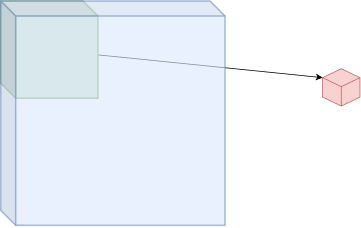
\includegraphics[width=0.7\textwidth]{pic/kernel2.png}
\end{center}

\end{frame}

%------------------------------------------slide55
\begin{frame}{SVM Gaussian Kernel: Example}

\begin{center}
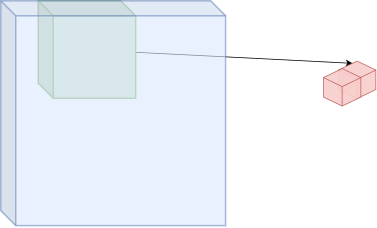
\includegraphics[width=0.7\textwidth]{pic/kernel3.png}
\end{center}

\end{frame}

%------------------------------------------slide56
\begin{frame}{SVM Gaussian Kernel: Example}

\begin{center}
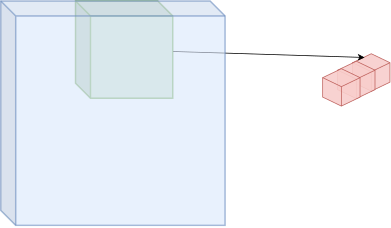
\includegraphics[width=0.7\textwidth]{pic/kernel4.png}
\end{center}

\end{frame}

%------------------------------------------slide57
\begin{frame}{SVM Gaussian Kernel: Example}

\begin{center}
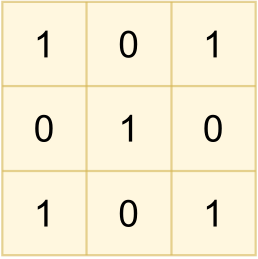
\includegraphics[width=0.7\textwidth]{pic/kernel5.png}
\end{center}

\end{frame}
%------------------------------------------slide58
\begin{frame}{SVM Gaussian Kernel: Example}

\begin{center}
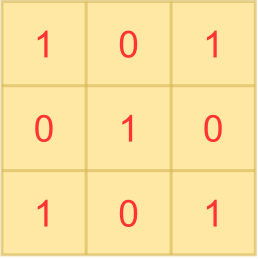
\includegraphics[width=0.7\textwidth]{pic/kernel6.png}
\end{center}

\end{frame}
%------------------------------------------slide59
\begin{frame}{Contributions}
\begin{itemize}
\item \textbf{This slide has been prepared thanks to:}
\begin{itemize}
\item \href{https://github.com/Mahdi-Aghaei}{Mahdi Aghaei}
    % \setlength{\itemsep}{10pt} % Adjust the value to control the spacing
    % \item \href{https://github.com/Mahan-Bayhaghi}{Mahan Bayhaghi}
\end{itemize}
\end{itemize}

\end{frame}

\begin{frame}[allowframebreaks]
    \bibliography{ref}
    \bibliographystyle{ieeetr}
    \nocite{*}
\end{frame}

\end{document}